
%(BEGIN_QUESTION)
% Copyright 2012, Tony R. Kuphaldt, released under the Creative Commons Attribution License (v 1.0)
% This means you may do almost anything with this work of mine, so long as you give me proper credit

Tolk trykkmålingen som vises av dette manometeret, forutsatt en nøyaktighet på $\pm$ 2\% av full skala:

$$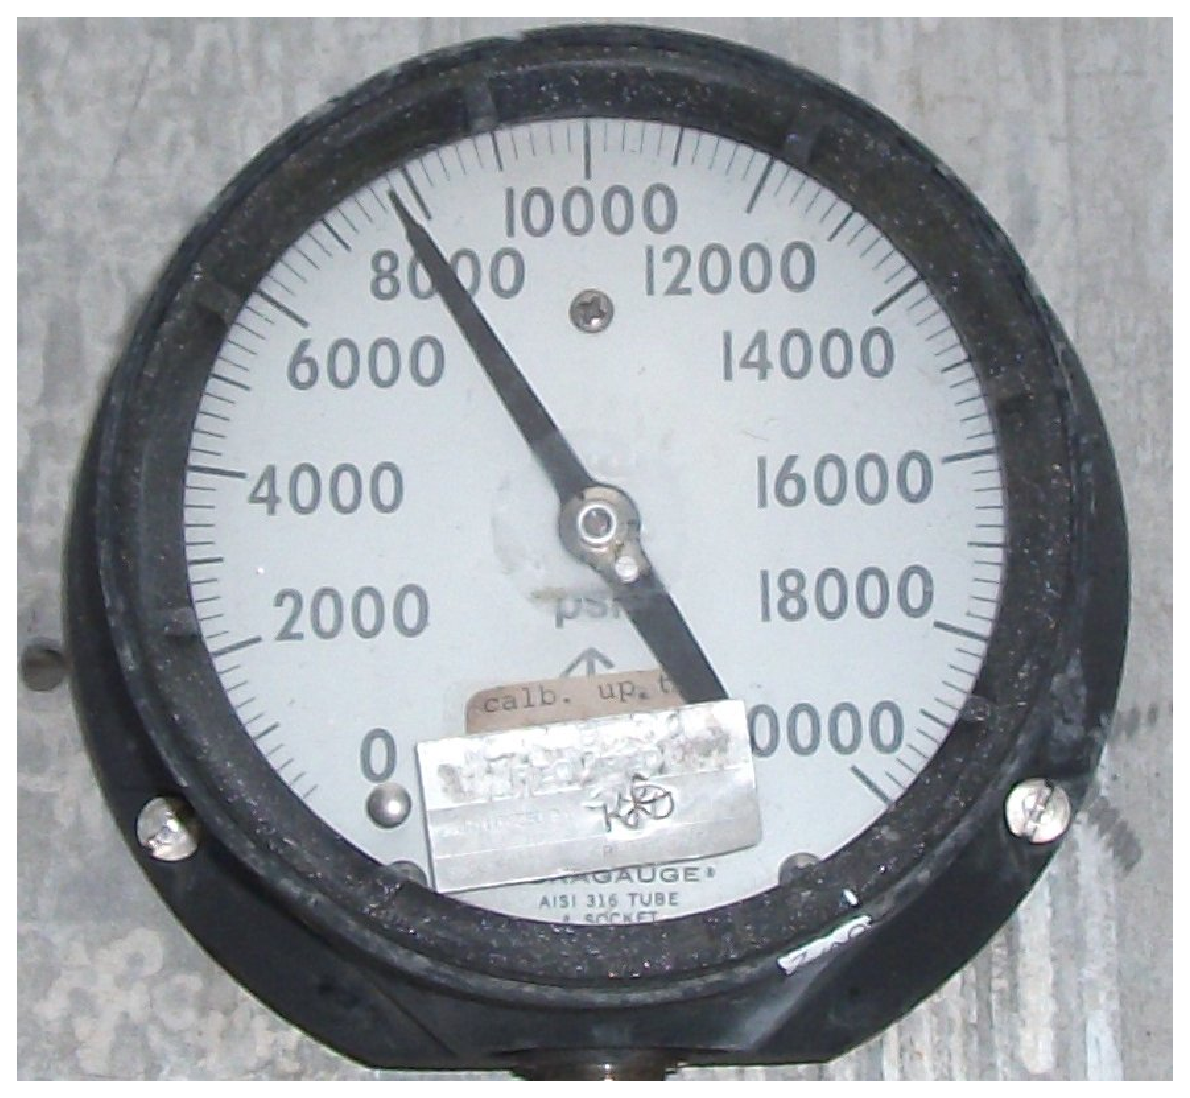
\includegraphics[width=15.5cm]{i01153x01.eps}$$

Hvor lavt og hvor høyt kan trykket faktisk være, gitt oppgitt nøyaktighet for dette manometeret?

\underbar{file i01153}
%(END_QUESTION)





%(BEGIN_ANSWER)

Trykk = 7800 PSI $\pm$ 400 PSI
 
\vskip 10pt

Det betyr at det faktiske trykket kan være så lavt som 7400 PSI eller så høyt som 8200 PSI.

%(END_ANSWER)





%(BEGIN_NOTES)


%INDEX% Measurement, analog gauge reading

%(END_NOTES)


